\documentclass{article}
\usepackage[english]{babel}
\usepackage[letterpaper,top=2cm,bottom=2cm,left=3cm,right=3cm,marginparwidth=1.75cm]{geometry}

% Useful packages
\usepackage{amsmath}
\usepackage{graphicx}
\usepackage[colorlinks=true, allcolors=blue]{hyperref}

\title{Research 1 Technical Report}
\author{Jayden Lombardi \\
Champlain College \\
jayden.lombardi@mymail.champlain.edu}

\begin{document}
\maketitle

\section{Overview}
The goal of this project is to make a simple "Hello World" base project program for the Nintendo 3DS using devkitPro and devkitARM tools, writing in C. This program will display text on screen based on button input, and will also have a toggleable strobe mode. This project will provide insight into base-level DS programming, and allow for users to expand upon and create any program or game they would like to load onto their DS. 

\subsection{Objectives}
\begin{enumerate}
\item Display "Hello [Button]" based on the button pressed; A, B, X, Y
\item Move a pixel on the top screen that corresponds with the D-Pad
\item Reset everything on the screen when left bumper is pressed
\end{enumerate}

With Adequate Time:
\begin{enumerate}
\item Display "Hello [Button]" At the current location of the pixel
\item Move a pixel on the bottom screen that corresponds with the Joystick
\item Left bumper resets everything to a black screen, pixel is now white
\item Right bumper resets everything to a white screen, pixel is now black
\end{enumerate}

\subsection{Application Functionality:}
\begin{enumerate}
    \item Touch and dragging on touchscreen will draw a white line
    \item Pressing SELECT button will toggle Strobe mode on and off - other commands can still be used during strobe mode
    \item Pressing A button will load an image of link on the bottom screen
    \item Pressing B button will clear everything on screen
    \item Pressing START button will quit the program
\end{enumerate}

\subsection{Why?}
Why are we researching this? Why are we coding to a 3DS?

\noindent Primarily, it is an exploration of the Nintendo 3DS, it's architecture and devkitPro tools. It is a look into how the Nintendo 3DS handles instructions, memory, display and user input/output. This project will provide valuable insight into how to link code, and how the C language translates user input into interactive outputs on screen. Learning how to store button states and access said data for conditional branches. It will serve as the base research for a programmer looking to get their hands dirty in Assembly, Linking, devkitPro and learn a bit more about gaming consoles and how they run.


\section{Implementation}
\subsection{Environment}
\begin{itemize}
\item ARM assembly for the 3DS - ARM instructions + memory management
\item Visual Studios 2022 for writing Assembly and C code
\item MSYS2 to compile and debug code
\item Citra to debug and test on laptop before switching to 3ds
\item Luma3DS and homebrew to homebrew my 3DS
\item My personal jail-broken 3DS for testing and debugging
\item 3DS Internal registers and memory 
\item SD Card and SD card reader to transfer files to 3DS from Laptop
\end{itemize}

\subsection{Tools}
\begin{enumerate}
\item Initialization
    \begin{itemize}
    \item Set up 3DS internal registers to prepare for button inputs
    \item Zero out and clear out any previously held data
    \end{itemize}
\item User Input Handling
    \begin{itemize}
    \item Involves checking a specific memory address
    \item Each button as well as the touch screen corresponds to a memory address, the value changes when the button is pressed
    \end{itemize}
\item Outputting to Display
    \begin{itemize}
    \item Output is done after input is handled
    \item Have an output Hello function and an output Character function
    \item Make sure output to the correct buffer
    \end{itemize}
\item Reset Functionality
    \begin{itemize}
    \item Clear display memory
    \item Setting background color to white
    \end{itemize}
\end{enumerate}


\section{Challenges and Solutions}
1 = Problem \newline
2 = Solution

\subsection{Macro}
\begin{itemize}
\item Understanding Nintendo 3DS Architecture
    \begin{enumerate}
    \item One major problem will definitely be understanding the Nintendo 3DS architecture. I have the smallest bit of experience with architectures in general, and this is all brand new for me. The 3DS uses ARM which I am not too familiar with, but will gain. The 3DS has specific memory-mapped input and output set ups, which I will need to become accustomed to. 
    \item I will need to research and study both ARM documentation and the unique set up of registers and memory in the 3DS. Carefully dealing and altering the 3DS memory, testing and debugging each function separately to verify each part of the code works. 
    \end{enumerate}
\item Limited Debugging
    \begin{enumerate}
    \item The 3DS does not have a built in debugger to help me debug the problems with my code. To make matters worse, most common debuggers are not compatible with a 3DS. 
    \item Using an emulation system on my laptop (Citra and MSYS2 in tandem) to observe how the memory and registers are changing when the code is stepped through. 
    \end{enumerate}
\item Setting up and Linking devkitPro and devkitARM
    \begin{enumerate}
        \item The problem I struggled with the most in this entire project was correctly setting up and linking the devkitPro tools, and the 3ds library to my project. This step took about 4 days in total of consistent work on the project. I was attempting to manually link and create a project through devkitPro. This meant manually setting paths, manually creating a Visual Studio project and directory, and attempting to link the library to it from devkitARM. This process threw numerous errors at me across multiple days, all of which I researched and preserved through. 
        \item The solution in the end was a single link online to someone else with the same exact problem (see \hyperref[micro5]{Micro 5}). There was a single response to the forum post, and it explained the devkitARM comes with pre-built pre-linked example projects. I felt very stupid not looking for these examples from the start but chose to persevere anyway. I made a copy of the most basic example and saw where the fault lied in my previous linking. After finally having a working environment to code and compile in after 4 days I was ecstatic. 
    \end{enumerate}
\end{itemize}

\subsection{Micro}
\begin{itemize}
\item Managing Registers Efficiently and Correctly
    \begin{enumerate}
    \item There are limited General purpose registers, and it is a good idea to use the intended registers for their intended purposes. Excessive loading to one register will slow down the program.
    \item Once again, I am not too familiar with ARM or the ARM registers, and do not know the most efficient way to go about using them. Planning on and researching the best way to use registers will be of great use to my project. As well as searching my code for excessive loading and storing areas.  
    \end{enumerate}
\item Memory Management for Display
    \begin{enumerate}
    \item More specifically the 3DS memory management for display. The last graphics programming class I took, I struggled a bit in grasping a few of the concepts. The 3DS has it's own system for managing display, that I will have to address correctly. 
    \item Refreshing my brain on graphics programming will help get a good general knowledge of display management. Researching specifically 3DS management on the Nintendo website will help me get accustomed to specifically displaying things to the 3DS screen. 
    \end{enumerate}
\item Displaying an Image on Screen
    \begin{enumerate}
        \item Another big but specific problem I faced was loading an image to the screen. I spent about 2-3 days on this before I had to call it quits and continue with the production, it was something I really wanted but was almost unable to complete. I was attempting to load a png on the bottom screen of the 3ds, but the 3ds does not accept png's so I had to switch the format of the image (see \hyperref[micro4]{Micro 4}). I tested multiple different for loops, as well as multiple different images to load to the bottom screen. Multiple times the images would load with incorrect colors, incorrect format, and compressed heavily either vertically or horizontally. In the end, the final image loaded is the furthest I was able to achieve. 
        \item In the end I never was able to fix it 100 percent. The image of Link loads but it is compressed and rotated 90 degrees counterclockwise. I ruled out a problem with the colors through the RGBtoRGB565 function, and removed the offset so it would just print in the top left corner. After this the solution was simply to try numerous different for-loop iterations, and find the one that worked best. In the end I was left with the double for-loop (see \hyperref[forloop]{Code Explanations}). I believe the function to also be a bit specific to this image, as others do not load correctly. In the future, I would really like to sort this out, I believe with more time it is within my ability to do so.  
    \end{enumerate}
\item \label{micro4} Putting Image Into correct format
    \begin{enumerate}
        \item As stated in the previous problem, finding and setting the correct format for the image being loaded was just as (if not more) important as the code used to load to the buffer. I needed to research the 3DS architecture to find and understand what type of file, size, color format, endian system, and depth the console uses when loading images. If any of these values were slightly off I would not know the source of the errors, from the image format or the code? I went through a wide range of file types (.bin, .sgi, .txt) before settling on .RAW. After settling on this it still took about a day to find an application that would format the image correctly. 
        \item The solution in the end was installing and making use of MagickImage (see \hyperref[immag]{ImgMagick}). Through this program I was able to open the command prompt terminal and convert any png I wish, while also setting every bit of information myself within the terminal. This allowed me to personally create and format the RAW file so it would accurately fit and match the 3DS architecture. A very useful tool that I will most definitely use in the future. I ran the following line within command prompt to turn the image from a png to a correctly formatted RAW. \newline 
        \verb|magick "C:\devkitPro\assets\link.png"|\newline
        \verb|-resize 320x240 -depth 8 -endian LSB RGB:link.raw|
    \end{enumerate}
\item \label{micro5} Cannot Find 3dsxcrt0.o
    \begin{enumerate}
        \item After spending about 4 days of attempting to correctly link devkit tools and the libctru 3DS library, I was blessed to fall upon \href{https://devkitpro.org/viewtopic.php?t=8997}{This} link. Similar to the post I was getting the continuous error that the application was unable to find the file \verb|"3dsx_crt0.o"| even though that file did indeed exist. Both me and the forum poster thought it was due to the fact that devkitPro was looking in the wrong directory for the file, so we both copied and pasted the crt0.o file into the correct directory. After doing so, I received an error that every function within the 3DS libctru library used VFP register arguments while my code did not. I spent about half a day trying to fix this, attempting to change paths and formatting of all of my current files. I was completely unsuccessful and went to the SmartSPACE programming tutor for help. 
        \item After about an hour in the SmartSPACE scratching my head I decided to look up the exact issue of the crt0.o file. After finally finding the forum post, I saw that the problem was the fact that the tutorial I was following was almost out of date, and 3DS homebrew code has greatly improved since it first started. The solution was found from a response underneath the forum, explaining that I should use the official devkitPro examples to start base code. This indeed worked! And although I spent 4 days trying to link the application I believe I learned a lot more about how devkitPro works in general, and it aided me in solving problems down the road.
    \end{enumerate}
\end{itemize}



\section{Code Explanations}

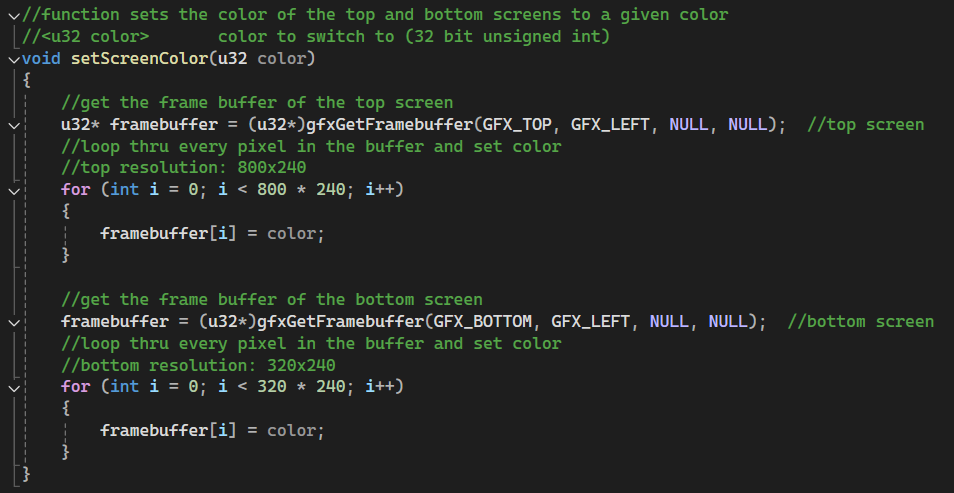
\includegraphics[width=0.75\linewidth]{image.png}     %Set Color 
    \begin{itemize}
        \item Function used to set the color of both screens to the input 'color'
        \item First the top screen frame buffer is pulled
        \item Then each pixel on the screen is set to the color (resolution 800x240)
        \item Second the bottom screen frame buffer is pulled
        \item Then each pixel on the screen is set to the color (resolution 320x240)
    \end{itemize}
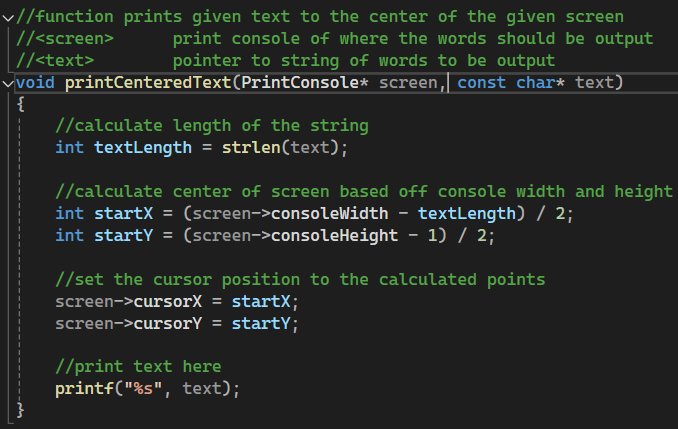
\includegraphics[width=0.75\linewidth]{image2.png}    %Print Text
    \begin{itemize}
        \item Functioned used to print text in the center of a given screen
        \item First string length is calculated
        \item Then center of the screen is calculated based on console width and height, and how long the text is
        \item Cursor is set to the position and text is printed
    \end{itemize}
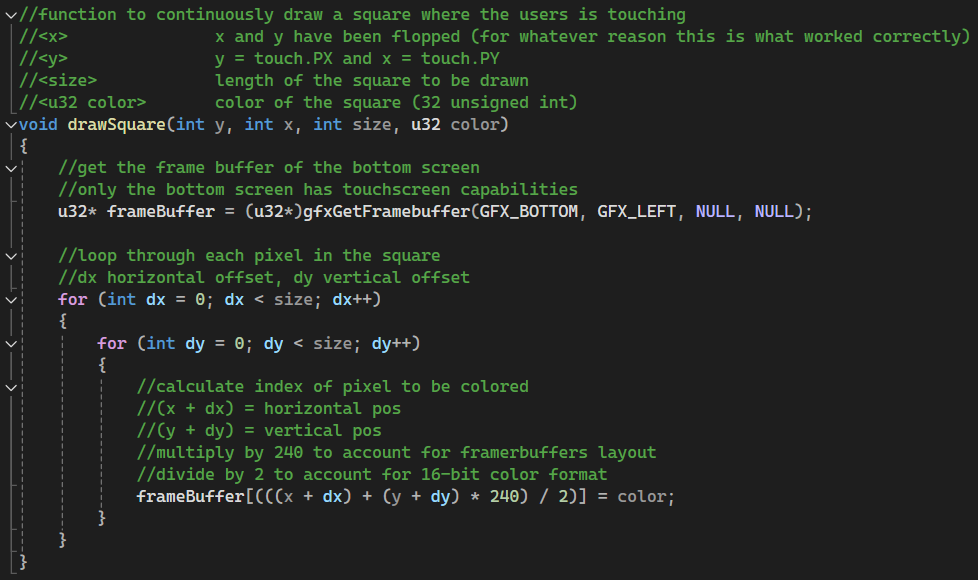
\includegraphics[width=0.75\linewidth]{image3.png}    %Draw Line
    \begin{itemize}
        \item Function used to continuously draw a square on the touchscreen
        \item Square is drawn at the given x, y value with the given size and color
        \item First bottom screen is pulled (only screen with touchscreen capabilities)
        \item Each pixel on the screen is looped through
        \item Calculate where the square should be currently drawn and add it to the framebuffer
    \end{itemize}
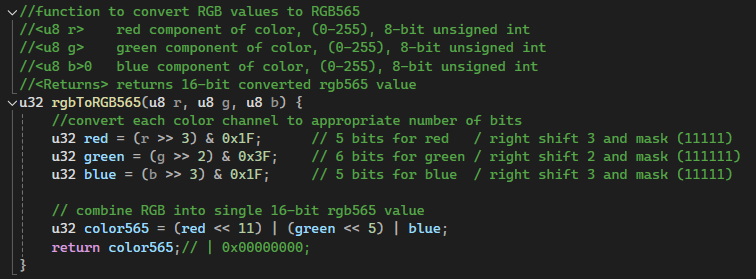
\includegraphics[width=0.75\linewidth]{image7.png}
    \begin{itemize}
        \item Function to switch from RGB to RGB565 given r,g,b values
        \item 5 bits for red = right shift 3
        \item 6 bits for green = right shift 2
        \item 5 bits for blue = right shift 3
        \item Then combine into single 16 bit value and return
    \end{itemize}
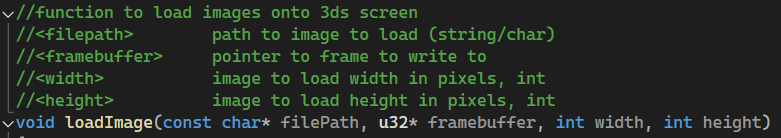
\includegraphics[width=0.75\linewidth]{image4.png}    %Load Image Sign.
    \begin{itemize}
        \item Signature of the function used to load a given image
        \item Filepath is path to the image on the sd card
        \item Framebuffer is pointer to which screen to write to
        \item Width and Height of the given image in pixels
    \end{itemize}
 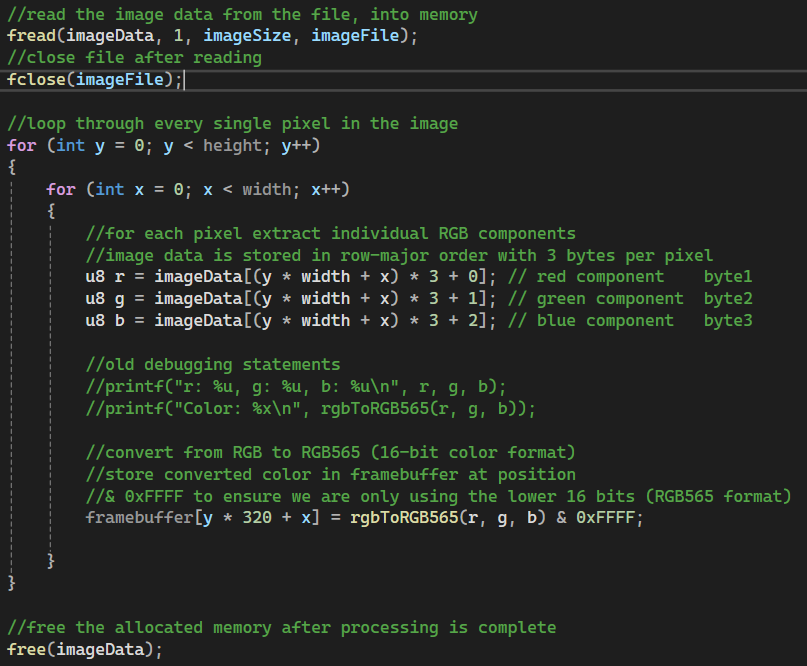
\includegraphics[width=0.75\linewidth]{image5.png}    %Load Image Logic
    \begin{itemize}  
        \item \label{forloop} Logic for loading the image to the screen
        \item First open the image data in fread, read from file into memory
        \item Close the image file after reading to not corrupt
        \item Then loop through each pixel in the image
        \item For each pixel extract the u8 r g and b values (3 bytes per pixel)
        \item Use the RGBtoRGB565 to convert to 16 bit color format
        \item Store converted color in framebuffer at pixel, only using the lower bits
    \end{itemize}
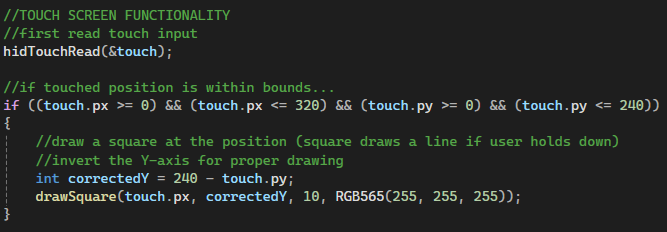
\includegraphics[width=0.75\linewidth]{image6.png}    %TouchScreen Func
    \begin{itemize}
        \item Logic within the main loop for touchscreen capabilities
        \item First read the touch input through hidTouchRead();
        \item If the touched position is within bounds of the lower screen draw the square at the given position
        \item correctedY is used to invert the y-axis so it draw properly. 
    \end{itemize}


\section{Future Plans}
Ideas and projects I am going to pursue over winter break as I really enjoyed the creation of this project: 

\begin{enumerate}
\item Display text at the current location of the pixel
\item Linking DPAD controls to movement
\item Linking Joystick controls to movement
\item Left bumper resets everything to a black screen, Right bumper resets to a white screen
\item Get any audio file to play
\item Get the 3 Dimensional aspect of the top screen working
\item Change the colors of the LEDs on the bottom of the 3DS
\item Correctly load an Image
\item Basic animations/textures
\end{enumerate}


\section{Reflection}
All i all yada yadfa yada
Things to improve upon:
\begin{enumerate}
    \item Rah
    \item Rah2
\end{enumerate}

\section{Sources}
\begin{itemize}
    \item DevKitPro Resources:
    \begin{enumerate}
        \item \href{https://devkitpro.org/wiki/Getting_Started}{DevKit Installation}
        \item \href{https://devkitpro.org/wiki/devkitPro_pacman}{DevKit Pacman Inst.}
        \item \href{https://gbatemp.net/threads/setup-a-devkitpro-environment-on-windows.652238/}{Setting up DevkitPro environment - Windows}
        \item \href{https://github.com/devkitPro/libctru}{DevKit 3ds Library Github}
        \item \href{https://devkitpro.org/viewtopic.php?t=8997}{No Such File or Directory FIX - DevkitPro}
        \item \href{https://www.youtube.com/watch?v=FNZVHvmGOIE}{HomeBrew YouTube Tutorial}
    \end{enumerate}

    \item MSYS2 Installation:
    \begin{enumerate}
        \item \href{https://www.msys2.org/wiki/MSYS2-installation/}{Official MSYS2 Website Install}
        \item \href{https://gbatemp.net/threads/install-msys-environment.652234/}{Install MSYS2 Environment}
    \end{enumerate}

    \item Citra Resources:
    \begin{enumerate}
        \item \href{https://citra-emulator.com/download/windows/}{Citra Official Install}
        \item \href{https://docs.libretro.com/library/citra/#google_vignette}{Citra Gen Info}
        \item I have previously used Citra to emulate Pokemon games online, and knew somewhat how the emulator worked!
    \end{enumerate}

    \item ImageMagick Resources:
    \begin{enumerate}
        \item\label{immag} \href{https://imagemagick.org/script/download.php}{ImageMagick Official Install}
        \item \href{https://imagemagick.org/script/convert.php}{ImageMagick Commands}
        \item \href{https://stackoverflow.com/questions/29120768/imagemagick-convert-png-16-bit-to-raw}{Stack Overflow ImageMagick}
    \end{enumerate}
\end{itemize}



\end{document}